% !TEX TS-program = lualatex
% !BIB TS-program = biber
%\documentclass[handout]{beamer}
\documentclass{beamer}
\input{../common/misomva}
\newcommand{\misoclasstinytitleslide}{Partially based on material by:  Branislav Kveton, \\[-1em] 
Mikhail Belkin, Jerry Zhu}
\newcommand{\misoclassdate}{}
\begin{document}
% Topic-specific title slide
\newcommand{\topictitle}{SSL Learnability}
\newcommand{\topicsubtitle}{When Does Graph-Based SSL Provably Help?}
\renewcommand{\misoclasstinytitleslide}{Partially based on material by:  Branislav Kveton, \\[-1em] Mikhail Belkin, Jerry Zhu}

\MakeTopicSlide

\begin{frame}
\frametitle{SSL with Graphs: What is behind it?}

\questionbox{Why and when it helps?} \pause
\moveb
\questionbox{Can we guarantee benefit of SSL over SL?} \pause
\moveb
\questionbox{Are there cases when \emphcol{manifold} SSL is provably helpful?} \pause
\moveb

Say $\cX$ is supported on manifold $\cM$. Compare two cases:
\smallskip
\begin{itemize}[<+-| alert@+>]\addtolength{\itemsep}{0.5\baselineskip}
\item SL: does not know about $\cM$ and only knows $(\bx_i,y_i)$
\item SSL: perfect knowledge of $\cM$ \pause $\equiv$ humongous amounts of $\bx_i$
\end{itemize}
\bigskip
{\tiny \url{http://people.cs.uchicago.edu/~niyogi/papersps/ssminimax2.pdf}}

\end{frame}
%%%%%%%%%%%%%%%%%%%%%%%%%%%%%%%%%%%%%%%%%%%%%%%%%%%%%%%%%%%%
\begin{frame}
\frametitle{SSL with Graphs: What is behind it?}

Set of learning problems - collections $\cP$ of probability distributions:

\[
\cP \pause = \cup_\cM \cP_\cM \pause  = \cup_\cM  \{p \in \cP | p_\cX \mbox{ is uniform on } \cM \}
\]

\begin{center}
% TikZ replacement for niyogicircles
\begin{tikzpicture}
    % M1: Perfect circle
    \draw (0,0) circle (1.5cm);
    \node at (0, 1.8) {\large \textbf{+1}};
    \node at (0, -1.8) {\large \textbf{-1}};
    \draw[thick] (-1.6, 0) -- (-1.4, 0); 
    \draw[thick] (1.4, 0) -- (1.6, 0);   
    \node at (0, -2.5) {\Large $\mathbf{M_1}$};
    % M2: Deformed circle
    \begin{scope}[xshift=6cm]
        \draw [smooth cycle] plot coordinates {
            (0.4, 1.2) (1.3, 1.0) (1.4, 0.3) (1.2, -0.5) (0, -1.5)
            (-1.2, -0.5) (-1.4, 0.3) (-1.3, 1.0) (-0.4, 1.2) (0, 0.8)
        };
        \node at (0, 1.6) {\large \textbf{-1}};
        \node at (0, -1.0) {\large \textbf{+1}};
        \draw[thick] (-1.6, -0.1) -- (-1.3, 0.0);
        \draw[thick] (1.4, 0.5) -- (1.7, 0.6);
        \node at (0, -2.5) {\Large $\mathbf{M_2}$};
    \end{scope}
\end{tikzpicture}
\end{center}

\end{frame}
%%%%%%%%%%%%%%%%%%%%%%%%%%%%%%%%%%%%%%%%%%%%%%%%%%%%%%%%%%%%
\begin{frame}
\frametitle{SSL with Graphs: What is behind it?}

\textbf{Set of problems}
$\cP = \cup_\cM \cP_\cM   = \{p \in \cP | p_\cX \mbox{ is uniform on } \cM \}$ \\
\pause
\textbf{Regression function} $m_p = \EEc{y}{x}$ when $x \in \cM$ \\
\pause
\textbf{Algorithm} $A$ and \textbf{labeled examples} 
$ \bar z = \{z_i\}_{i=1}^{n_l} = \{(\bx_i,y_i)\}_{i=1}^{n_{l}}$ \\
\pause
\textbf{Minimax rate}

\[
R(n_{l},\cP) = \mcolA{\inf_A}\ \sup_{p \in \cP} \EEs{\bar z}{\|A(\bar z) - m_p\|_{L^2(p_\bX)}}
\]
\pause
Since $\cP = \cup_\cM \cP_\cM$
\pause
\[
R(n_{l},\cP) = \mcolA{\inf_A}\ \mcolB{\sup_\cM} \sup_{p \in \cP_\cM} \EEs{\bar z}{\|A(\bar z) - m_p\|_{L^2(p_\bX)}}
\]
\pause
(SSL) When $A$ is allowed to know $\cM$ \pause
\[
Q(n_{l},\cP) = \mcolB{\sup_\cM} \ \mcolA{\inf_A} \sup_{p \in \cP_\cM} \EEs{\bar z}{\|A(\bar z) - m_p\|_{L^2(p_\bX)}}
\] \pause
\rightquestionbox{In which cases there is a gap between $Q(n_{l},\cP)$ and $R(n_{l},\cP)$?}
\end{frame}
%%%%%%%%%%%%%%%%%%%%%%%%%%%%%%%%%%%%%%%%%%%%%%%%%%%%%%%%%%%%
\begin{frame}
\frametitle{SSL with Graphs: What is behind it?}

\textbf{Hypothesis space} $\cH$: half of the circle as $+1$ and the rest as $-1$

\begin{center}
\resizebox{0.75\columnwidth}{!}{%
\begin{tikzpicture}[scale=1.2]
    
    % === M1: Circle manifold (left) ===
    \begin{scope}[xshift=0cm]
        % Main circle
        \draw[thick] (0,0) circle (2cm);
        
        % Tick marks crossing through the curve (perpendicular)
        \draw[thick] (-2.15,0) -- (-1.85,0);
        \draw[thick] (2.15,0) -- (1.85,0);
        
        % Labels +1 (top) and -1 (bottom)
        \node[font=\large] at (0,2.5) {$+1$};
        \node[font=\large] at (0,-2.5) {$-1$};
        
        % M1 label
        \node[font=\large] at (0,-3.5) {$M_1$};
    \end{scope}
    
    % === M2: Irregular blob manifold (right) - apple/heart shape ===
    \begin{scope}[xshift=7cm]
        % Apple/heart-like blob shape with indent at top
        \draw[thick] 
            (0,-2) % bottom center (+1 position)
            .. controls (-1.2,-2.1) and (-2,-1.5) .. (-1.9,-0.5) % left side lower
            .. controls (-1.8,0.3) and (-1.6,1) .. (-1.2,1.5) % left side upper
            .. controls (-0.8,1.9) and (-0.5,2.1) .. (-0.3,1.7) % left lobe going to indent
            .. controls (-0.1,1.3) and (0.1,1.3) .. (0.3,1.7) % indent dip at top center
            .. controls (0.5,2.1) and (0.9,2.2) .. (1.4,1.8) % right lobe
            .. controls (1.9,1.4) and (2.2,0.8) .. (2.1,0.2) % right side upper
            .. controls (2,-.4) and (1.8,-1.2) .. (1.4,-1.7) % right side lower
            .. controls (1,-2.1) and (0.5,-2.1) .. (0,-2); % back to bottom
        
        % Tick marks crossing through the curve (perpendicular to curve direction)
        % Left tick: crosses at (-1.85, -0.1) area
        \draw[thick] (-2.1,-0.1) -- (-1.6,-0.1);
        % Right tick: crosses at upper right around (2.05, 0.5) area  
        \draw[thick] (1.85,0.65) -- (2.25,0.35);
        
        % Labels -1 (top) and +1 (bottom)
        \node[font=\large] at (0,2.5) {$-1$};
        \node[font=\large] at (0,-2.8) {$+1$};
        
        % M2 label
        \node[font=\large] at (0,-3.5) {$M_2$};
    \end{scope}
    
\end{tikzpicture}
}
\end{center}
\smallskip
\pause
\textbf{Case 1:} $\cM$ is known to the learner ($\cH_\cM$)
\bigskip
\pause
\questionbox{What is a VC dimension of $\cH_\cM$?}
\pause
\onslide<handout:0>{2}
\pause
\[ 
\mbox{Optimal rate } Q(n,\cP) \leq 2 \sqrt{\frac{3 \log n_{l}}{n_{l}}}
\]


\end{frame}
%%%%%%%%%%%%%%%%%%%%%%%%%%%%%%%%%%%%%%%%%%%%%%%%%%%%%%%%%%%%
\begin{frame}
\frametitle{SSL with Graphs: What is behind it?}
\textbf{Case 2:} $\cM$ is \emphcol{unknown} to the learner 
\pause
\[
R(n_{l},\cP) = \mcolA{\inf_A} \sup_{p \in \cP} \EEs{\bar z}{\|A(\bar z) - m_p\|_{L^2(p_\bX)}} = \pause \Omega\left( 1 \right)
\]
\pause
We consider $2^d$ manifolds of the form
\[
\cM = \mbox{Loops} \cup \mbox{Links} \cup C \mbox{ where } C = \cup_{i=1}^d C_i 
\]
\begin{center}
\resizebox{0.55\columnwidth}{!}{%
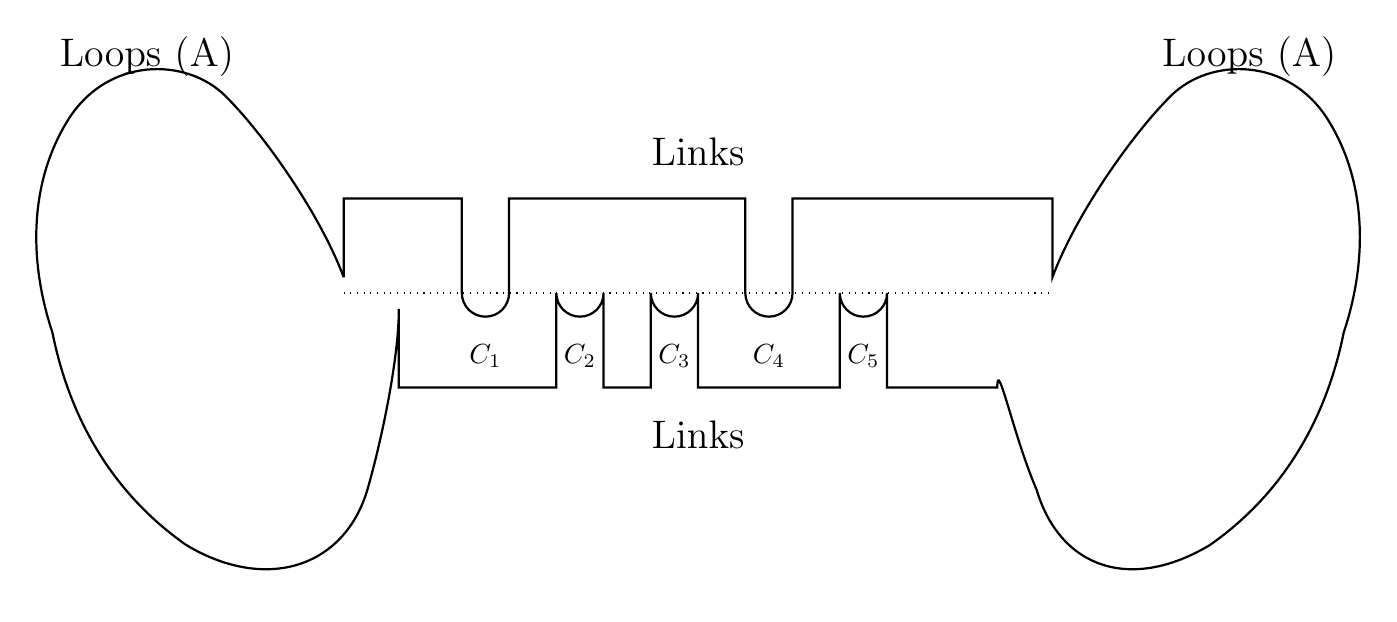
\begin{tikzpicture}[scale=1.0]

    % Configuration
    \def\TopY{1.2}
    \def\BotY{-1.2}
    \def\MidY{0} % The alignment line
    
    % Draw continuous boundary
    \draw[thick]
        % === LEFT BLOB ===
        (-4.5, 0.2)
        .. controls (-4.8, 1.0) and (-5.5, 2.0) .. (-6.0, 2.5)
        .. controls (-6.5, 3.0) and (-7.5, 3.0) .. (-8.0, 2.2)
        .. controls (-8.5, 1.4) and (-8.5, 0.4) .. (-8.2, -0.5)
        .. controls (-8.0, -1.5) and (-7.5, -2.5) .. (-6.5, -3.2)
        .. controls (-5.5, -3.8) and (-4.5, -3.5) .. (-4.2, -2.5)
        .. controls (-4.0, -1.8) and (-3.8, -0.8) .. (-3.8, -0.2)
        
        % === BOTTOM BOUNDARY (Left to Right) ===
        -- (-3.8, \BotY) -- (-3.0, \BotY)
        
        % C1 (Top Dip region): Bottom is straight
        -- (-2.4, \BotY)
        
        % C2 (Bottom Block): Corners at y=0
        -- (-1.8, \BotY) -- (-1.8, 0)
        arc[start angle=180, end angle=360, radius=0.3]
        -- (-1.2, \BotY)
        
        % C3 (Bottom Block)
        -- (-0.6, \BotY) -- (-0.6, 0)
        arc[start angle=180, end angle=360, radius=0.3]
        -- (0.0, \BotY)
        
        % C4 (Top Dip region): Bottom is straight
        -- (1.2, \BotY)
        
        % C5 (Bottom Block)
        -- (1.8, \BotY) -- (1.8, 0)
        arc[start angle=180, end angle=360, radius=0.3]
        -- (2.4, \BotY)
        
        -- (3.8, \BotY)
        
        % === RIGHT BLOB ===
        .. controls (3.8, -0.8) and (4.0, -1.8) .. (4.3, -2.5)
        .. controls (4.6, -3.5) and (5.5, -3.8) .. (6.5, -3.2)
        .. controls (7.5, -2.5) and (8.0, -1.5) .. (8.2, -0.5)
        .. controls (8.5, 0.4) and (8.5, 1.4) .. (8.0, 2.2)
        .. controls (7.5, 3.0) and (6.5, 3.0) .. (6.0, 2.5)
        .. controls (5.5, 2.0) and (4.8, 1.0) .. (4.5, 0.2)
        
        % === TOP BOUNDARY (Right to Left) ===
        -- (4.5, \TopY)
        -- (2.4, \TopY)
        
        % C5 region: Top is straight
        -- (1.8, \TopY)
        
        % C4 (Top Dip): Corners at y=0
        -- (1.2, \TopY) -- (1.2, 0)
        arc[start angle=0, end angle=-180, radius=0.3]
        -- (0.6, \TopY)
        
        % C3 region: Top is straight
        -- (0.0, \TopY)
        
        % C2 region: Top is straight
        -- (-1.2, \TopY)
        
        % C1 (Top Dip): Corners at y=0
        -- (-2.4, \TopY) -- (-2.4, 0)
        arc[start angle=0, end angle=-180, radius=0.3]
        -- (-3.0, \TopY)
        
        -- (-4.5, \TopY)
        -- (-4.5, 0.2)
        ;

    % Center Dotted Line at EXACTLY y=0
    \draw[dotted] (-4.5, 0) -- (4.5, 0);

    % Labels
    \node[font=\Large] at (-7, 3) {Loops (A)};
    \node[font=\Large] at (7, 3) {Loops (A)};
    \node[font=\Large] at (0, 1.8) {Links};
    \node[font=\Large] at (0, -1.8) {Links};

    % C Labels
    \node at (-2.7, -0.8) {$C_1$};
    \node at (-1.5, -0.8) {$C_2$};
    \node at (-0.3, -0.8) {$C_3$};
    \node at (0.9, -0.8) {$C_4$};
    \node at (2.1, -0.8) {$C_5$};

\end{tikzpicture}
}
\end{center}
\pause
\begin{flushright}
\textbf{Main idea}: $d$ segments in $C$, $d-l$ with no data,
$2^l$ possible choices for labels, which 
helps us to lower bound $\|A(\bar z) - m_p\|_{L^2(p_\bX)}$
\end{flushright}
\end{frame}
%%%%%%%%%%%%%%%%%%%%%%%%%%%%%%%%%%%%%%%%%%%%%%%%%%%%%%%%%%%%
\begin{frame}
\frametitle{SSL with Graphs: What is behind it?}
\begin{center}
\resizebox{0.6\columnwidth}{!}{%
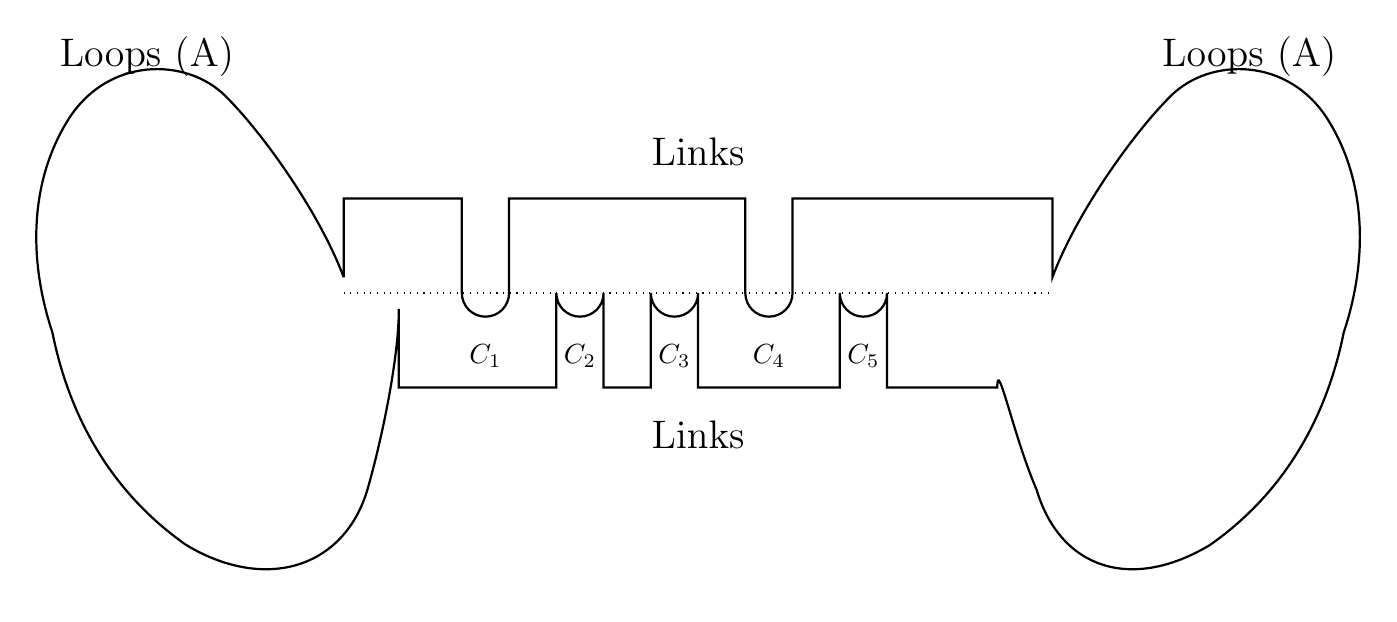
\begin{tikzpicture}[scale=1.0]

    % Configuration
    \def\TopY{1.2}
    \def\BotY{-1.2}
    \def\MidY{0} % The alignment line
    
    % Draw continuous boundary
    \draw[thick]
        % === LEFT BLOB ===
        (-4.5, 0.2)
        .. controls (-4.8, 1.0) and (-5.5, 2.0) .. (-6.0, 2.5)
        .. controls (-6.5, 3.0) and (-7.5, 3.0) .. (-8.0, 2.2)
        .. controls (-8.5, 1.4) and (-8.5, 0.4) .. (-8.2, -0.5)
        .. controls (-8.0, -1.5) and (-7.5, -2.5) .. (-6.5, -3.2)
        .. controls (-5.5, -3.8) and (-4.5, -3.5) .. (-4.2, -2.5)
        .. controls (-4.0, -1.8) and (-3.8, -0.8) .. (-3.8, -0.2)
        
        % === BOTTOM BOUNDARY (Left to Right) ===
        -- (-3.8, \BotY) -- (-3.0, \BotY)
        
        % C1 (Top Dip region): Bottom is straight
        -- (-2.4, \BotY)
        
        % C2 (Bottom Block): Corners at y=0
        -- (-1.8, \BotY) -- (-1.8, 0)
        arc[start angle=180, end angle=360, radius=0.3]
        -- (-1.2, \BotY)
        
        % C3 (Bottom Block)
        -- (-0.6, \BotY) -- (-0.6, 0)
        arc[start angle=180, end angle=360, radius=0.3]
        -- (0.0, \BotY)
        
        % C4 (Top Dip region): Bottom is straight
        -- (1.2, \BotY)
        
        % C5 (Bottom Block)
        -- (1.8, \BotY) -- (1.8, 0)
        arc[start angle=180, end angle=360, radius=0.3]
        -- (2.4, \BotY)
        
        -- (3.8, \BotY)
        
        % === RIGHT BLOB ===
        .. controls (3.8, -0.8) and (4.0, -1.8) .. (4.3, -2.5)
        .. controls (4.6, -3.5) and (5.5, -3.8) .. (6.5, -3.2)
        .. controls (7.5, -2.5) and (8.0, -1.5) .. (8.2, -0.5)
        .. controls (8.5, 0.4) and (8.5, 1.4) .. (8.0, 2.2)
        .. controls (7.5, 3.0) and (6.5, 3.0) .. (6.0, 2.5)
        .. controls (5.5, 2.0) and (4.8, 1.0) .. (4.5, 0.2)
        
        % === TOP BOUNDARY (Right to Left) ===
        -- (4.5, \TopY)
        -- (2.4, \TopY)
        
        % C5 region: Top is straight
        -- (1.8, \TopY)
        
        % C4 (Top Dip): Corners at y=0
        -- (1.2, \TopY) -- (1.2, 0)
        arc[start angle=0, end angle=-180, radius=0.3]
        -- (0.6, \TopY)
        
        % C3 region: Top is straight
        -- (0.0, \TopY)
        
        % C2 region: Top is straight
        -- (-1.2, \TopY)
        
        % C1 (Top Dip): Corners at y=0
        -- (-2.4, \TopY) -- (-2.4, 0)
        arc[start angle=0, end angle=-180, radius=0.3]
        -- (-3.0, \TopY)
        
        -- (-4.5, \TopY)
        -- (-4.5, 0.2)
        ;

    % Center Dotted Line at EXACTLY y=0
    \draw[dotted] (-4.5, 0) -- (4.5, 0);

    % Labels
    \node[font=\Large] at (-7, 3) {Loops (A)};
    \node[font=\Large] at (7, 3) {Loops (A)};
    \node[font=\Large] at (0, 1.8) {Links};
    \node[font=\Large] at (0, -1.8) {Links};

    % C Labels
    \node at (-2.7, -0.8) {$C_1$};
    \node at (-1.5, -0.8) {$C_2$};
    \node at (-0.3, -0.8) {$C_3$};
    \node at (0.9, -0.8) {$C_4$};
    \node at (2.1, -0.8) {$C_5$};

\end{tikzpicture}
}
\end{center}

\textbf{Knowing the manifold helps}
\begin{itemize}[<+-| alert@+>]%\addtolength{\itemsep}{0.5\baselineskip}
\item $C_1$ and $C_4$ are close 
\item $C_1$ and $C_3$ are far
\item we also need: \emphcol{target function varies smoothly}
\item altogether: \textbf{closeness on manifold $\to$ similarity in labels}
\end{itemize}

\end{frame}
%%%%%%%%%%%%%%%%%%%%%%%%%%%%%%%%%%%%%%%%%%%%%%%%%%%%%%%%%%%%
\begin{frame}
\frametitle{SSL with Graphs: What is behind it?}
\questionbox{What does it mean to \emphcol{know $\cM$}?}
\moveb
\pause
\textbf{Different degrees of knowing $\cM$}
\begin{itemize}%\addtolength{\itemsep}{0.5\baselineskip}
\item set membership oracle: $\bx \stackrel{?}{\in} \cM$
\item approximate oracle
\item knowing the harmonic functions on $\cM$
\item knowing the Laplacian $\cL_\cM$
\item knowing eigenvalues and eigen\emph{functions} 
\item topological invariants, e.g., dimension
\item metric information: geodesic distance
\end{itemize}
\end{frame}
%%%%%%%%%%%%%%%%%%%%%%%%%%%%%%%%%%%%%%%%%%%%%%%%%%%%%%%%%%%%



\MakeLastSlide
\end{document}
